\documentclass[]{article}
\usepackage[T1]{fontenc}
\usepackage{lmodern}
\usepackage{amssymb,amsmath}
\usepackage{ifxetex,ifluatex}
\usepackage{fixltx2e} % provides \textsubscript
% use upquote if available, for straight quotes in verbatim environments
\IfFileExists{upquote.sty}{\usepackage{upquote}}{}
\ifnum 0\ifxetex 1\fi\ifluatex 1\fi=0 % if pdftex
  \usepackage[utf8]{inputenc}
\else % if luatex or xelatex
  \ifxetex
    \usepackage{mathspec}
    \usepackage{xltxtra,xunicode}
  \else
    \usepackage{fontspec}
  \fi
  \defaultfontfeatures{Mapping=tex-text,Scale=MatchLowercase}
  \newcommand{\euro}{€}
\fi
% use microtype if available
\IfFileExists{microtype.sty}{\usepackage{microtype}}{}
\usepackage[margin=1in]{geometry}
\usepackage{color}
\usepackage{fancyvrb}
\newcommand{\VerbBar}{|}
\newcommand{\VERB}{\Verb[commandchars=\\\{\}]}
\DefineVerbatimEnvironment{Highlighting}{Verbatim}{commandchars=\\\{\}}
% Add ',fontsize=\small' for more characters per line
\usepackage{framed}
\definecolor{shadecolor}{RGB}{248,248,248}
\newenvironment{Shaded}{\begin{snugshade}}{\end{snugshade}}
\newcommand{\KeywordTok}[1]{\textcolor[rgb]{0.13,0.29,0.53}{\textbf{{#1}}}}
\newcommand{\DataTypeTok}[1]{\textcolor[rgb]{0.13,0.29,0.53}{{#1}}}
\newcommand{\DecValTok}[1]{\textcolor[rgb]{0.00,0.00,0.81}{{#1}}}
\newcommand{\BaseNTok}[1]{\textcolor[rgb]{0.00,0.00,0.81}{{#1}}}
\newcommand{\FloatTok}[1]{\textcolor[rgb]{0.00,0.00,0.81}{{#1}}}
\newcommand{\CharTok}[1]{\textcolor[rgb]{0.31,0.60,0.02}{{#1}}}
\newcommand{\StringTok}[1]{\textcolor[rgb]{0.31,0.60,0.02}{{#1}}}
\newcommand{\CommentTok}[1]{\textcolor[rgb]{0.56,0.35,0.01}{\textit{{#1}}}}
\newcommand{\OtherTok}[1]{\textcolor[rgb]{0.56,0.35,0.01}{{#1}}}
\newcommand{\AlertTok}[1]{\textcolor[rgb]{0.94,0.16,0.16}{{#1}}}
\newcommand{\FunctionTok}[1]{\textcolor[rgb]{0.00,0.00,0.00}{{#1}}}
\newcommand{\RegionMarkerTok}[1]{{#1}}
\newcommand{\ErrorTok}[1]{\textbf{{#1}}}
\newcommand{\NormalTok}[1]{{#1}}
\usepackage{graphicx}
% Redefine \includegraphics so that, unless explicit options are
% given, the image width will not exceed the width of the page.
% Images get their normal width if they fit onto the page, but
% are scaled down if they would overflow the margins.
\makeatletter
\def\ScaleIfNeeded{%
  \ifdim\Gin@nat@width>\linewidth
    \linewidth
  \else
    \Gin@nat@width
  \fi
}
\makeatother
\let\Oldincludegraphics\includegraphics
{%
 \catcode`\@=11\relax%
 \gdef\includegraphics{\@ifnextchar[{\Oldincludegraphics}{\Oldincludegraphics[width=\ScaleIfNeeded]}}%
}%
\ifxetex
  \usepackage[setpagesize=false, % page size defined by xetex
              unicode=false, % unicode breaks when used with xetex
              xetex]{hyperref}
\else
  \usepackage[unicode=true]{hyperref}
\fi
\hypersetup{breaklinks=true,
            bookmarks=true,
            pdfauthor={},
            pdftitle={Contenido},
            colorlinks=true,
            citecolor=blue,
            urlcolor=blue,
            linkcolor=magenta,
            pdfborder={0 0 0}}
\urlstyle{same}  % don't use monospace font for urls
\setlength{\parindent}{0pt}
\setlength{\parskip}{6pt plus 2pt minus 1pt}
\setlength{\emergencystretch}{3em}  % prevent overfull lines
\setcounter{secnumdepth}{5}

%%% Change title format to be more compact
\usepackage{titling}
\setlength{\droptitle}{-2em}
  \title{Contenido}
  \pretitle{\vspace{\droptitle}\centering\huge}
  \posttitle{\par}
  \author{}
  \preauthor{}\postauthor{}
  \date{}
  \predate{}\postdate{}




\begin{document}

\maketitle


{
\hypersetup{linkcolor=black}
\setcounter{tocdepth}{2}
\tableofcontents
}
\section{Rápida introducción a RStudio y a
Rmarkdown}\label{rapida-introduccion-a-rstudio-y-a-rmarkdown}

\subsection{Para empezar}\label{para-empezar}

Antes de empezar lo que tenéis que hacer es instalar en vuestro
ordenador personal:

\begin{itemize}
\itemsep1pt\parskip0pt\parsep0pt
\item
  Una \href{http://cran.es.r-project.org/}{versión reciente de R}.
\item
  La \href{http://www.rstudio.com/products/rstudio/download/}{última
  versión de Rstudio Desktop v0.98.1073}
\item
  Si queréis todas las funcionalidades deberéis instalar algunos
  programas adicionales como
  \href{http://latex-project.org/ftp.html}{TeX/LaTeX}.
\item
  Los demás programas necesarios suelen estar instalados en un ordenador
  personal.
\end{itemize}

Si ya teníais una versión de R o de Rstudio debéis actualizarla. Algunos
de los programas que utilizaremos son muy recientes y sólo se instalaran
(en particular Rmarkdown) si os actualizáis a una versión de Rstudio
Desktop \textgreater{}= v0.98.1073.

\subsection{Rstudio básico}\label{rstudio-basico}

Los autores de \href{http://www.rstudio.com/}{RStudio}, entre otras
cosas, nos proporcionan el programa RStudio Desktop que es un entorno de
desarrollo integrado (\emph{IDE}). Es decir es un entorno de
programación que consiste en un editor de código, utilidades de
compilación (ejecución de código), etc. Vamos que es la más exitosa
interfaz gráfica de usuario (\emph{GUI}) que nos permite trabajar de
forma cómoda con R.

Además dispone de una serie de utilidades para la generación de informes
de una forma ágil y sencilla.

En en la propia web de Rstudio tenéis unos fantásticos manuales sobre
esta aplicación.

Aquí explicamos lo más básico, lo demás lo aprenderéis de forma
intuitiva o leyendo las lecciones del cursos, los manuales y consultando
con los compañeros en los foros.

Esta es, posiblemente, la primera vista de RStudio

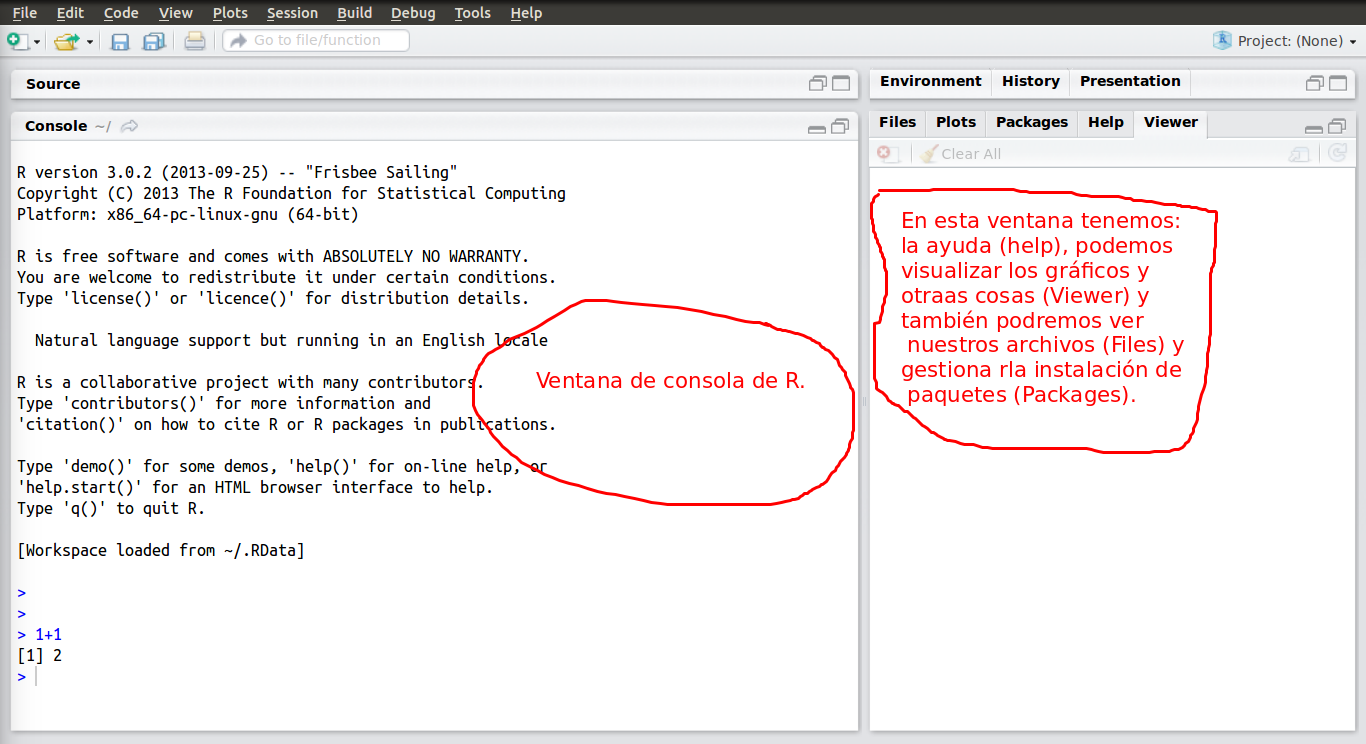
\includegraphics{figures/RStudioInicio1.png}

En el menú File podéis abrir un R Script (y entre otras cosas un fichero
de Rmarkdown) como se ve en el siguiente gráfico

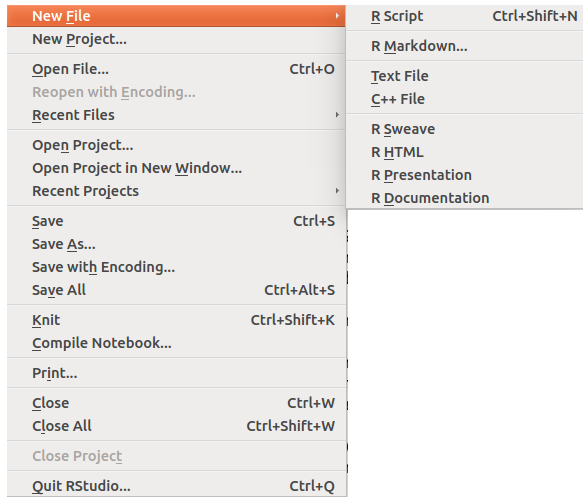
\includegraphics{figures/Menu_Inicio1.png}

La situación después de abrir un R Script es la siguiente

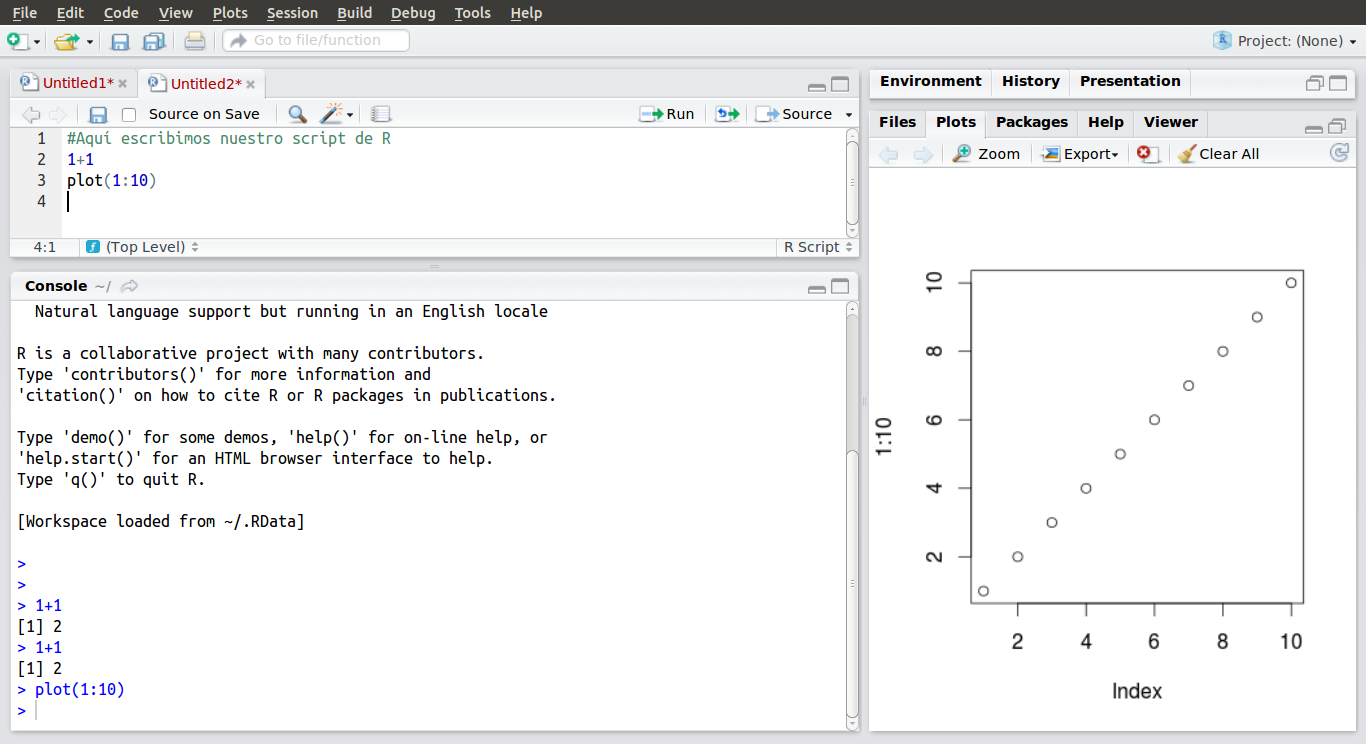
\includegraphics{figures/RStudio_RScript1.png}

\subsection{Rmarkdown básico}\label{rmarkdown-basico}

Para lo que queremos que aprendáis este curso el \emph{Markdown Quick
Reference} es suficiente. Pero os tenemos que ayudar un poco más con las
fórmulas matemáticas, el formato que se puede dar a las \emph{chunks} de
R.

\subsection{Fórmulas matemáticas en R markdown
}\label{formulas-matematicas-en-r-markdown}

La manera de introducir fórmulas matemáticas en \texttt{R Markdown}
sigue una sintaxis similar a la de del sistema de composición de textos
científicos LaTeX. Si habéis utilizado Moodle seguramente habréis visto
utilizar a algunos alumnos y profesores esta menera de escribir en
fórmulas. De hecho esta capacidad la tiene Moodle pues tiene activado su
propio lenguaje markdown.

No tiene ningún misterio. Solo tenemos que introducir un código que
representa la fórmula de dos formas:

\begin{enumerate}
\def\labelenumi{\arabic{enumi}.}
\itemsep1pt\parskip0pt\parsep0pt
\item
  Para las fórmulas o ecuaciones en una misma línea (\emph{inline
  equations}) se pone el código entre dos dobles dólares:
  \texttt{\$código\$}
\item
  Para las fórmulas o ecuaciones entre líneas (\emph{display equations})
  se pone el código entre dos dólares: \texttt{\$\$código\$\$}
\end{enumerate}

A continuación se muestran algunos ejemplos de código:

\subsection{Fórmulas}\label{formulas}

\textbf{Letras griegas, símbolos y acentos matemáticos}

\begin{itemize}
\itemsep1pt\parskip0pt\parsep0pt
\item
  Código:
  \texttt{\$\textbackslash{}mu, \textbackslash{}beta, \textbackslash{}lambda, \textbackslash{}sigma, \textbackslash{}Sigma\$}
\item
  Salida: $\mu,\beta,\lambda,\sigma,  \Sigma$
\item
  Código:
  \texttt{\$\textbackslash{}tilde\{S\}, \textbackslash{}overline\{x\},  \textbackslash{}overline\{X\}, \textbackslash{}hat\{p\}\$}
\item
  Salida: $\tilde{S}, \overline{x},  \overline{X}, \hat{p}$
\item
  Código:
  \texttt{\$\textbackslash{}infty, -\textbackslash{}infty,  +\textbackslash{}infty, \textbackslash{}pm\textbackslash{}infty\$}
\item
  Salida: $\infty, -\infty,  +\infty, \pm\infty$
\end{itemize}

Subíndices, superíndices, comparaciones:

\begin{itemize}
\itemsep1pt\parskip0pt\parsep0pt
\item
  Código: \texttt{\$x\_\{i\}\$}
\item
  Salida: $x_{i}$
\item
  Código: \texttt{\$x\^{}\{25\}\$}
\item
  Salida: $x^{25}$
\item
  Código: \texttt{\$x\_\{i j\}\$}
\item
  Salida: $x_{i j}$
\item
  Código:
  \texttt{\$x\^{}\{2\textbackslash{}cdot \textbackslash{}alpha\}, \textbackslash{}tilde\{S\}\^{}2,\textbackslash{}sqrt\{x\}\$}
\item
  Salida: $x^{2\cdot \alpha}, \tilde{S}^2, \sqrt{x}$
\item
  Código: \texttt{\$\textbackslash{}mu=\textbackslash{}mu\_\{0\}\$}
\item
  Salida: $\mu=\mu_{0}$
\item
  Código: \texttt{\$3.141516\textbackslash{}approx 3.14\$}
\item
  Salida: $3.141516\approx 3.14$
\item
  Código:
  \texttt{\$\textbackslash{}mu\textbackslash{}neq \textbackslash{}mu\_\{0\}\$}
\item
  Salida: $\mu\neq \mu_{0}$
\item
  Código:
  \texttt{\$\textbackslash{}mu \textgreater{} \textbackslash{}mu\_\{0\}, \textbackslash{}mu\textbackslash{}geq \textbackslash{}mu\_\{0\}\$}
\item
  Salida: $\mu > \mu_{0}, \mu\geq \mu_{0}$
\item
  Código:
  \texttt{\$\textbackslash{}mu \textless{} \textbackslash{}mu\_\{0\}, \textbackslash{}mu\textbackslash{}leq \textbackslash{}mu\_\{0\}\$}
\item
  Salida: $\mu < \mu_{0}, \mu\leq \mu_{0}$
\end{itemize}

\textbf{Fracciones} * Código:
\texttt{\$\textbackslash{}frac\{\textbackslash{}alpha\}\{2\}\$} *
Salida: $\frac{\alpha}{2}$ * Código:
\texttt{\$z\_\{1-\textbackslash{}frac\{\textbackslash{}alpha\}\{2\}\}, 8\^{}\{\textbackslash{}frac\{1\}\{3\}\}\$}
* Salida: $z_{1-\frac{\alpha}{2}}, 8^{\frac{1}{3}}$ * Código:
\texttt{\$\textbackslash{}frac\{\textbackslash{}tilde\{S\}\}\{\textbackslash{}sqrt\{n\}\}\$}
* Salida: $\frac{\tilde{S}}{\sqrt{n}}$

\textbf{Paréntesis, corchetes y llaves}:

\begin{itemize}
\itemsep1pt\parskip0pt\parsep0pt
\item
  Simples. Código:
  \texttt{\$(a,b); {]}a,b{[}; \textbackslash{}\{a,b\textbackslash{}\}\$}
\item
  Salida: $(a,b); ]a,b[; \{a,b\}$
\item
  Que se adaptan al tamaño
  \texttt{\textbackslash{}left(\textbackslash{}right)},\texttt{\textbackslash{}left{]}\textbackslash{}right{]}}\ldots{}
\end{itemize}

Código:

\begin{verbatim}
$\left[\overline{X} -z_{1-\frac{\alpha}{2}} \frac{\sigma}{\sqrt{n}}, \overline{X}+z_{1-\frac{\alpha}{2}}\frac{\sigma}{\sqrt{n}}
\right]$
\end{verbatim}

Salida:

\[\left[\overline{X} -z_{1-\frac{\alpha}{2}} \frac{\sigma}{\sqrt{n}}, \overline{X}+z_{1-\frac{\alpha}{2}}\frac{\sigma}{\sqrt{n}}
\right]\]

\subsection{Matrices }\label{matrices}

Las matrices se definen empezando con
\texttt{\textbackslash{}begin\{array\}\{lcr\}} y acabando con
\texttt{\textbackslash{}end\{array\}}. La letras \texttt{lcr} entre
llaves indican tanto el número de columnas como si se alinean a
izquierda (\textbf{l}eft), derecha (\textbf{r}ight) o quedan centradas
(\textbf{c}enter). Entre el
\texttt{\textbackslash{}begin\{array\}\{lcl\}} y el
\texttt{\textbackslash{}end\{array\}} se introducen por filas los
valores de la matriz separados por el símbolo \texttt{\&} y el cambio de
fila se indica con \texttt{\textbackslash{}\textbackslash{}}. En
principio las matrices contienen fórmulas. Si queremos introducir texto
en una fórmula tenemos que crear una caja de texto con la instrucción
\texttt{\textbackslash{}mbox\{ pon aquí tu texto\}} (\texttt{mbox} es el
la abreviatura de \emph{make a box})

\begin{verbatim}
$
\left(
\begin{array}{ll}
123 & 4 \\
1   & 234
\end{array}
\right)
$
\end{verbatim}

Salida:

\[
\left(
\begin{array}{ll}
123 & 4 \\
1   & 234
\end{array}
\right)
\]

\begin{verbatim}
$
\left\{
\begin{array}{ll}
123 & 4 \\
1   & 234\mbox{ dato atípico}
\end{array}
\right\}
$
\end{verbatim}

Salida:

\[
\left\{
\begin{array}{ll}
123 & 4  \\
1   & 234 \mbox{ dato atípico}
\end{array}
\right\}
\]

Si queremos eliminar una llave del lado derecho hay que escribir

\begin{verbatim}
\left\{\right.
\end{verbatim}

\emph{Notad que el punto de} \texttt{\textbackslash{}right.} es el que
indica se tiene que omitir la llave (o paréntesis o corchete) derecha.
Por ejemplo

\begin{verbatim}
$$
\left\{
\begin{array}{ll}
123 & 4  \\
1   & 234 \mbox{ dato atípico}
\end{array}
\right.
$$
\end{verbatim}

Salida:

\[
\left\{
\begin{array}{ll}
123 & 4  \\
1   & 234 \mbox{ dato atípico}
\end{array}
\right.
\]

\subsection{Contrastes de hipótesis }\label{contrastes-de-hipotesis}

Ahora unas plantillas ejemplo para escribir los contrastes de hipótesis:

En la misma línea que el texto.

\begin{itemize}
\item
  Código: Contrastaremos la hipótesis nula
  \texttt{\$H\_\{0\}: \textbackslash{}mu=\textbackslash{}mu\_0\$} contra
  la alternativa bilateral
  \texttt{\$H\_\{1\}: \textbackslash{}mu\textbackslash{}neq\textbackslash{}mu\_0\$}.
\item
  Salida: Contrastaremos la hipótesis nula $H_{0}: \mu=\mu_0$ contra la
  alternativa bilateral $H_{1}: \mu\neq\mu_0$.
\end{itemize}

Con el modo \emph{fórmulas entre líneas}

Código: Vamos a realizar el siguiente contraste

\begin{verbatim}
$$
\left\{
\begin{array}{ll}
H_{0}: &  \mu=\mu_0\\
H_{1}: & \mu\neq\mu_0
\end{array}
\right.
$$
\end{verbatim}

Salida:

Vamos a realizar el siguiente contraste

\[
\left\{
\begin{array}{ll}
H_{0}: &  \mu=\mu_0\\
H_{1}: & \mu\neq\mu_0
\end{array}
\right.
\]

\subsection{Parámetros de las \emph{chunks} de R
}\label{parametros-de-las-chunks-de-r}

Sabemos que las \emph{chunks} de R se indican

```

\begin{Shaded}
\begin{Highlighting}[]
\NormalTok{x=}\DecValTok{1+1}  
\NormalTok{x }
\end{Highlighting}
\end{Shaded}

\begin{verbatim}
## [1] 2
\end{verbatim}

```

La parte entre llaves que empieza por r puede contener diversos
parámetros que son opcionales. Por ejemplo

```

\begin{Shaded}
\begin{Highlighting}[]
\NormalTok{x=}\DecValTok{1+1}  
\NormalTok{x}
\end{Highlighting}
\end{Shaded}

```

NUEVO

La primera es una etiqueta o nombre que tendrá la \emph{chunk}, y está
formada por un blanco que lo separa de la r seguido por una cadena de
caracteres sin blancos, las demás opciones viene separadas por comas. Si
no se desea poner etiqueta y sí opciones se pone ```\{r , opciones\}.

\begin{itemize}
\itemsep1pt\parskip0pt\parsep0pt
\item
  La opción \texttt{echo} es lógica e indica si se muestra
  (\texttt{TRUE} que es valor por defecto) o no (\texttt{FALSE}) el
  código fuente de R.
\item
  La opción \texttt{results} a la que podemos asignar:
\item
  El valor `markup' que es la opción por defecto y muestra los
  resultados en el documento
\item
  El valor `hide' que no muestra los resultados.
\item
  Dispone de otros valores que no comentamos.
\end{itemize}

Los siguientes ejemplos ilustran el comportamiento de estas opciones

La opción por defecto es la que \textbf{muestra todo}, tanto el código
como los resultados.

```\{r todo\_se\_ve, echo=TRUE,results=`markup'\}`\\x=1+1\\x\\```

\begin{Shaded}
\begin{Highlighting}[]
\NormalTok{x=}\DecValTok{1+1}
\NormalTok{x}
\end{Highlighting}
\end{Shaded}

\begin{verbatim}
## [1] 2
\end{verbatim}

Para que se vea \textbf{solamente el código}

```\{r solo\_codigo, echo=TRUE,results=`hide'\}\\x=1+1\\x\\```

\begin{Shaded}
\begin{Highlighting}[]
\NormalTok{x=}\DecValTok{1+1}
\NormalTok{x}
\end{Highlighting}
\end{Shaded}

Para que se vean \emph{solamente los resultados} y no el código

```\{r solo\_resultados, echo=FALSE,results=`markup'\}\\x=1+1\\x\\```

\begin{verbatim}
## [1] 2
\end{verbatim}

Para que \emph{no se vea nada}, ni el resultado ni el código

```\{r no\_se\_ve\_nada, echo=FALSE,results=`hide'\}\\x=1+1\\x\\```

Y como se ve no se ve nada:-)

\subsection{Las \emph{chunks} en modo línea
}\label{las-chunks-en-modo-linea}

Las \emph{chunks} que hemos visto hasta ahora no permiten introducir
resultados dentro de una línea de texto. La sintaxis de Rmarkdown para
insertar resultados de código en una línea es `r código `.

Por ejemplo la \textbf{entrada}

El cubo de dos es `r 2\^{}3 `. O lo que es lo mismo \texttt{\$2\^{}3\$=}
`r 2\^{}3 `

produce la \textbf{salida}

El cubo de dos es 8. O lo que es lo mismo $2^3$=8

Veamos un ejemplo más práctico. Nos dan una muestra y nos piden calcular
la media, la varianza, la desviación típica y el tamaño muestral.
Primero cargamos los datos y hacemos los cálculos con una \emph{chunk}

\begin{Shaded}
\begin{Highlighting}[]
\NormalTok{muestra=}\KeywordTok{c}\NormalTok{(}\DecValTok{1}\NormalTok{,}\DecValTok{2}\NormalTok{,}\DecValTok{3}\NormalTok{,}\OtherTok{NA}\NormalTok{,}\FloatTok{2.8}\NormalTok{,}\FloatTok{3.1}\NormalTok{,}\FloatTok{4.9}\NormalTok{)}
\NormalTok{muestra}
\end{Highlighting}
\end{Shaded}

\begin{verbatim}
## [1] 1.0 2.0 3.0  NA 2.8 3.1 4.9
\end{verbatim}

\begin{Shaded}
\begin{Highlighting}[]
\NormalTok{media=}\KeywordTok{mean}\NormalTok{(muestra,}\DataTypeTok{na.rm=}\OtherTok{TRUE}\NormalTok{)}
\NormalTok{media}
\end{Highlighting}
\end{Shaded}

\begin{verbatim}
## [1] 2.8
\end{verbatim}

\begin{Shaded}
\begin{Highlighting}[]
\NormalTok{var=}\KeywordTok{var}\NormalTok{(muestra,}\DataTypeTok{na.rm=}\OtherTok{TRUE}\NormalTok{)}
\NormalTok{var}
\end{Highlighting}
\end{Shaded}

\begin{verbatim}
## [1] 1.684
\end{verbatim}

\begin{Shaded}
\begin{Highlighting}[]
\NormalTok{desv.tipica=}\KeywordTok{sd}\NormalTok{(muestra,}\DataTypeTok{na.rm=}\OtherTok{TRUE}\NormalTok{)}
\NormalTok{desv.tipica}
\end{Highlighting}
\end{Shaded}

\begin{verbatim}
## [1] 1.298
\end{verbatim}

\begin{Shaded}
\begin{Highlighting}[]
\NormalTok{n=}\KeywordTok{length}\NormalTok{(}\KeywordTok{na.omit}\NormalTok{(muestra))}
\NormalTok{n}
\end{Highlighting}
\end{Shaded}

\begin{verbatim}
## [1] 6
\end{verbatim}

El siguiente \textbf{código de entrada}

\begin{Shaded}
\begin{Highlighting}[]
\NormalTok{La muestra es de tamaño $n$}\ErrorTok{=}\StringTok{`}\DataTypeTok{r n}\StringTok{`}\NormalTok{, su media es $\textbackslash{}overline\{x\}$}\StringTok{ }\ErrorTok{=}\StringTok{`}\DataTypeTok{r media}\StringTok{`}\NormalTok{,}
\NormalTok{su varianza es $\textbackslash{}tilde\{s\}\textbackslash{}^}\DecValTok{2}\NormalTok{$}\ErrorTok{=}\StringTok{`}\DataTypeTok{r var}\StringTok{`} \NormalTok{y su desviación típica es  $\textbackslash{}tilde\{s\}$}\ErrorTok{=}\StringTok{`}\DataTypeTok{r desv.tipica}\StringTok{`}\NormalTok{.}
\end{Highlighting}
\end{Shaded}

produce la \textbf{salida}

La muestra es de tamaño $n$=6, su media es $\overline{x}$=2.8, su
varianza es $\tilde{s}^2$=1.684 y su desviación típica es
$\tilde{s}$=1.2977.

Con esto terminamos esta pequeña introducción de algunos pequeños
aspectos más avanzados de Rmarkdown. En futuras lecciones y talleres
iremos avanzando en otros aspectos. Más adelante, de momento no perdáis
el tiempo, daremos referencias a manuales avanzados.

\subsection{Presentación de tablas de
datos}\label{presentacion-de-tablas-de-datos}

Para prsentar de forma adecuada tablas de datos con R existen diversos
procedimientos.

Uno de los más sencillos es utilizar la librería `xtable Esta librería
convierte tablas de datos y data frames a html y LaTeX.

En primer lugar hay que instalar la librería y cargarla con

\begin{Shaded}
\begin{Highlighting}[]
\CommentTok{#Descomentar si no está instalada}
\CommentTok{#install.pakcages("xtable")}
\KeywordTok{library}\NormalTok{(xtable)}
\end{Highlighting}
\end{Shaded}

\end{document}
